\documentclass[addpoints,12pt]{exam}
\usepackage{amsmath, amssymb}
\linespread{1.1}
\usepackage{graphicx}
\usepackage{multirow}
\boxedpoints
\pointsinmargin
\usepackage[T5,T1]{fontenc}  


%\printanswers
\noprintanswers

\pagestyle{headandfoot}
\runningheadrule
\runningheader{Econ 103}
              {Final Examination, Page \thepage\ of \numpages}
              {December 11th, 2015}

\runningfooter{Name: \rule{5cm}{0.4pt}}{}{Student ID \#: \rule{5cm}{0.4pt}}


%%%%%%%%%%%%%%%%%%%%%%%%%%%%%%%%%%%%%%%%%%%%%%%%%%%%%%%%%%%%%%%
\begin{document}

\begin{center}
\large
\sc{Final Examination\\ \normalsize Econ 103, Statistics for Economists \\ \vspace{0.5em} December 11th, 2015}

\vspace{1em}

\normalsize
\fbox{\begin{minipage}{0.5\textwidth}
\textbf{You will have 120 minutes to complete this exam.
Graphing calculators, notes, and textbooks are not permitted. }\end{minipage}}


\end{center}
%%%%%%%%%%%%%%%%%%%%%%%%%%%%%%%%%%%%%%%%%%%%%%%%%%%%%%%%%%%%%%%


\vspace{2em}
\begin{center}
  \fbox{\fbox{\parbox{5.5in}{\centering
        I pledge that, in taking and preparing for this exam, I have abided by the University of Pennsylvania's Code of Academic Integrity. I am aware that any violations of the code will result in a failing grade for this course.}}}
\end{center}
\vspace{0.2in}
\makebox[\textwidth]{Name:\enspace\hrulefill}

\vspace{0.2in}
\noindent \makebox[\textwidth]{Student ID \#:\enspace\hrulefill}

\vspace{0.3in}
\noindent\makebox[\textwidth]{Signature:\enspace\hrulefill}

%\rule{1cm}{0.4pt}
\vspace{2em}

\begin{center}
  \gradetable[h][questions]
\end{center}

\vspace{2em}

\paragraph{Instructions:} Answer all questions in the space provided, continuing on the back of the page if you run out of space. Show your work for full credit but be aware that writing down irrelevant information will not gain you points. Be sure to sign the academic integrity statement above and to write your name and student ID number on \emph{each page} in the space provided. Make sure that you have all pages of the exam before starting.

\paragraph{Warning:} If you continue writing after we call time, even if this is only to fill in your name, twenty-five points will be deducted from your final score. In addition, two points will be deducted for each page on which you do not write your name and student ID. 

%%%%%%%%%%%%%%%%%%%%%%%%%%%%%%%%%%%%%%%%%%%%%%%%%%%%%%%%%%%%%%%
\newpage
\begin{questions}


 \question Mark each statement as TRUE or FALSE. If FALSE provide a one sentence explanation. 
 \begin{parts}
   \part[3] If $(2, 6)$ is a 95\% CI for $\mu$, we do not reject $H_0\colon \mu = 1$ vs.\ $H_A\colon \mu \neq 1$ with $\alpha=0.05$.
   \begin{solution}[0.5in]
     FALSE: we would reject $\mu=1$ since 1 lies outside the CI.
   \end{solution}
   \part[3] A Type I error is rejecting a false null hypothesis.  
   \begin{solution}[0.6in]
     FALSE: it is rejecting a \emph{true} null hypothesis.
   \end{solution}
 	\part[3] The smaller the p-value the stronger the evidence against $H_0$. 
  \begin{solution}[0.6in]
    TRUE
  \end{solution}
   \part[3] The power of a hypothesis test equals the probability of making a Type II error.
   \begin{solution}[0.6in]
     FALSE: it is one \emph{minus} the probability of making a type II error.
   \end{solution}
   \part[3] If $A$ and $B$ are mutually exclusive events then $P(A\cup B) = P(A) + P(B)$. 
   \begin{solution}[0.6in]
     TRUE
   \end{solution}
   \part[3] If $A$ and $B$ events such that $A$ implies $B$ then $P(A)\leq P(B)$.
   \begin{solution}[0.6in]
     TRUE
   \end{solution}
   \part[3] The concept of \emph{efficiency} involves comparing the MSE of biased estimators. 
   \begin{solution}[0.6in]
    FALSE: it involves comparing the \emph{variances} of \emph{unbiased} estimators.
  \end{solution}
 	\part[3] If $X$ is a continuous RV with pdf $f(x)$ then $f(0)$ gives $P(X=0)$.
  \begin{solution}[0.6in]
    FALSE: if $X$ is continuous $P(X=x)=0$ for any $x$.
  \end{solution}
  \part[3] If $X$ and $Y$ are two RVs, then $E[XY] = Cov(X,Y) + E[X]E[Y]$. 
  \begin{solution}[0.6in]
    TRUE
  \end{solution}
  \part[3] If $X$ and $Y$ are discrete RVs then $p_Y(y) = \sum_{\mbox{\scriptsize all } y} p_{XY}(x,y)$.
  \begin{solution}[0.6in]
    FALSE: the sum should be taken over all $x$.
  \end{solution}
 \end{parts}

 \question For each of the following, provide R code to generate the specified result. 
  \begin{parts} 
    \part[4] Suppose I have a dataframe called \texttt{gradebook} with a column called \texttt{midterm1}.
  Write down R code to display only those rows of \texttt{gradebook} for which the entry in \texttt{midterm1} is at least 80.
  \begin{solution}[1in]
    \begin{verbatim}
subset(gradebook, midterm1 >= 80)
    \end{verbatim}
  \end{solution}
  	\part[6] Write code to plot the CDF of a $\chi^2(5)$ RV from 0 to 10 over a grid of 1001 values.
    \begin{solution}[1.5in]
    \begin{verbatim}
x <- seq(from = 0, to = 10, by = 0.01)
y <- pchisq(x, df = 5)
plot(x, y, type = `l')
    \end{verbatim}
  \end{solution}
  		\part[5] Write code to create a vector containing 20 simulated rolls of a fair, six-sided die. 
      \begin{solution}[1.25in]
    Various possibilities, the simplest of which is
    \begin{verbatim}
sample(1:6, size = 20, replace = TRUE)
    \end{verbatim}
  \end{solution}
  \part[10] Write an R function called \texttt{my.rt} to make one random draw from the $t(\nu)$ distribution.
      Your function should take one input argument, the degrees of freedom \texttt{nu}, and return the random draw.
      In your answer you may use any R functions you like \emph{except} for \texttt{rt}.
      \begin{solution}[2.5in]
    \begin{verbatim}
my.rt <- function(nu){
  normal.draw <- rnorm(1)
  chisq.draw <- rchisq(1, nu)
  return(normal.draw / sqrt(chisq.draw / nu))
}
    \end{verbatim}
  \end{solution}
	 \end{parts}

\question This question concerns a game played by rolling a fair, six-sided die with sides numbered 1--6.
To play the game you roll the die once.
Let $x$ denote the number on the side that shows face-up.
If $x$ is even you win $x$ dollars but if $x$ is odd you win $2x$ dollars.
\begin{parts}
  \part[4] Suppose you were to play this game an extremely large number of times.
  On average, how much would you win per play?
  \begin{solution}[1.25in]
    The expected winnings in this game are
    $$\frac{1}{6}\left[ \left( 2 + 4 + 6 \right) + 2 \times \left( 1 + 3 + 5 \right) \right] = 30/6 = 5$$
    so you will win, on average, 5 dollars per play in a long sequence of plays.
  \end{solution}
  \part[6] Your winnings in one play of this game can be viewed as the realization of a discrete random variable $Z$. 
  Calculate $Var(Z)$.
  \begin{solution}[1.85in]
    By the Shortcut Formula $Var(Z) = E[Z^2] - E[Z]^2$.
    We have
    \begin{eqnarray*}
      E[Z^2] &=& \sum_{\mbox{all }z} z^2 p(z) = \frac{1}{6}\left[ (2^2 + 4^2 + 6^2) + (2 \times 1)^2 + (2 \times 3)^2 + (2 \times 5)^2 \right]\\
      &=& \frac{1}{6}\left[ \left( 4 + 16 + 36 \right) + \left( 2^2 + 6^2 + 10^2 \right) \right] = \frac{1}{6} \left[ 56 + \left( 4 + 36 + 100 \right) \right]\\ 
      &=& 196/6 
    \end{eqnarray*}
    Therefore $Var(Z) = 196/6 - 25 = 23/3 \approx 7.67$
  \end{solution}
  \part[10] Suppose you play this game 69 times consecutively.
  Based on the approximation provided by the CLT, roughly what is the probability that your average winnings will be less than \$4.34 per play?
  \begin{solution}[2in]
    Since individual throws of a fair die are independent and identically distributed we have $Z_1, \dots Z_{69} \sim \mbox{iid}$ with mean $5$ and variance $23/3$ by parts (a) and (b).
    The question asks us to approximate the value of $P(\bar{Z}<4.34)$ where $\bar{Z} = (Z_1 + \dots + Z_{69})/69$.
    By the CLT $\bar{Z}$ is approximately normally distributed with mean 5 and standard deviation $\sqrt{(23/3)/69} = 1/3$. 
    We have
    $$P(\bar{Z} < 4.34) = P\left( \frac{\bar{Z}-5}{1/3} < -1.98 \right) = \texttt{pnorm}(-1.98) \approx 0.025$$
  \end{solution}
\newpage
\uplevel{For rest of this question we change the rules of the game as follows: after rolling the die and observing $x$ you are given the option to roll a \emph{second time}.
  If you choose not to roll a second time, your winnings are calculated as before: $x$ dollars if $x$ is even and $2x$ dollars if $x$ is odd.
  If you \emph{do} choose to roll again your winnings are calculated in the same way but based on whatever number comes up on your \emph{second roll}. 
For example if your initial roll is 3 and you re-roll and get a 1 then you win 2 dollars.} 
\part[5] If you want to maximize your average winnings over a large number of plays of this \emph{modified} game, then you should choose to roll a second time if and only if your first roll is a 1, 2, or 4.
Briefly explain why.
\begin{solution}[2.5in]
   Using the same logic as in part (a) your expected payoff from the second roll is 5 dollars.
   Thus, you should re-roll if $x$ is such that you would win \emph{less} than 5 dollars by sticking with your first roll.
   Accordingly the strategy that maximizes your expected payoff is to stick with your first roll if it is a 3, 5, or 6 and to re-roll if it is a 1, 2, or 4. 
  \end{solution}
  \part[15] Nina played this game once following the strategy  given in the preceding part.
  She won 10 dollars.
  Given this information, what is the probability that she chose to roll the die a second time?
  \begin{solution}[3.5in]
    Let $A$ be the event that Nina chose to roll the die a second time and $B$ be the event that she won 10 dollars. 
    We are asked to calculate $P(A|B)$.
    By Bayes' Rule
    $$P(A|B)=\frac{P(B|A)P(A)}{P(B)}$$
    and by the Law of Total Probability
    \begin{eqnarray*}
      P(B) &=& P(B|A)P(A) + P(B|A^C)P(A^C)
    \end{eqnarray*}
    Using the strategy from the preceding part, Nina will re-roll if she gets a 1, 2, or 4 her initial roll.
    Thus, since the die is fair, $P(A) = 1/2$ so we have
    $$P(A|B)=\frac{P(B|A)}{P(B|A) + P(B|A^C)}$$
    Now, $P(B|A^C)$ is the probability that Nina won 10 dollars given that she did \emph{not} roll twice.
    Since she is following the strategy from part (d), if Nina does not roll twice then she must have rolled a 3, 5, or 6 initially. 
    Thus $P(B|A^C)=1/3$.
    Now, recall that if Nina rolls twice then her winnings depend on the second roll \emph{only}.
  This means that $P(B|A)$ equals the probability of winning 10 dollars in the \emph{original} version of the game from parts (a)--(c) above, namely 1/6. 
  Therefore $P(A|B) = (1/6)/(1/3 + 1/6) = 1/3$.
  If Nina wins 10 dollars it is more likely than not that she only rolled once.
  \end{solution}
  %\part If Nina play the game a very large number of times, always following the strategy from part (e), on average how much will she win per game? 
\end{parts}


\question Clayton wants to know the fraction of Penn students who come from Guam, a small western Pacific island, so he polls a random sample of 96: none come from Guam.
\begin{parts}
  \part[5] Apply the ``textbook'' procedure for constructing an approximate 95\% CI for a population proportion based on the CLT to the data given in the problem statement.
  \begin{solution}[2.3in]
    Since $\widehat{p}=0$, the textbook interval $\widehat{p} \pm \texttt{pnorm}(1 - \alpha/2)\sqrt{\widehat{p}(1-\widehat{p})/n}$ simply gives $(0,0)$.
  \end{solution}
  \part[5] Repeat the preceding part using the \emph{refined} interval.
  \begin{solution}[2.3in]
  To construct the refined 95\% interval we add four ``fake'' observations to the dataset: two zeros and two ones.
  This gives us a new dataset with 100 observations, two of which are ones so that $\widetilde{p} = 0.02$ and $\widetilde{n} = 100$ and the approximate 95\% interval is
  $$0.02 \pm 2\sqrt{0.02 \times 0.98/100}$$
  which gives $(-0.008, 0.048)$.
  \end{solution}
  \part[5] Compare and contrast the two intervals you constructed above.
  Which makes more sense and why?
  Briefly explain your answer. 
  \begin{solution}[2.3in]
    The textbook interval is nonsensical in this example: it implies that we have complete certainty that absolutely no one at Penn comes from Guam.
    This is a ridiculous conclusion to draw from the data we have.
    This is an example where the approximation from the CLT breaks down because the sample size is too small relative to the population proportion we are trying to estimate. (We would expect a priori that very few students at Penn come from Guam.) 
    The refined interval corrects this defect and provides a much more reasonable answer although, naturally, we shouldn't take the LCL literally since a population proportion cannot be negative! 
  \end{solution}
\end{parts}

\question Professor Quack has developed a diet plan where you are allowed to eat anything you want as long you wash down every meal with a spoonful of pickle juice.
He claims that if you follow this diet you will lose, on average, 3kg over 4 weeks.
Matt decides to carry out an experiment to test this claim.
He recruits a random sample of 25 subjects and puts all of them on the ``pickle juice diet.''
Let $X_i$ be person $i$'s weight (in kg) before beginning the diet and $Y_i$ be person $i$'s weight (in kg) after four weeks on the diet.
The summary statistics from Matt's experiment are as follows:

\vspace{1em}

\begin{tabular}
	{l|cc}
	&$X$&$Y$\\
	\hline
	Sample Mean & $83$ & $82$\\
	Sample S.D. & $6$ & $10$ \\
	Correlation & \multicolumn{2}{c}{$0.3$} 
\end{tabular}

\vspace{1em}

Throughout this question please work with the approximation provided by the CLT.
For simplicity you may treat this approximation as though it were exact.
\begin{parts}
  \part[3] Is this an independent samples or matched pairs problem? Explain in one sentence.
  \begin{solution}[1.25in]
    Matched pairs: we're interested in how much weight people lose over the course of the diet which involves a before-and-after comparison for each subject.
  \end{solution}
  \part[4] Let $L_i$ denote the (positive) amount of weight that subject $i$ lost over the course Matt's experiment: $L_i = X_i - Y_i$.
  Calculate $\bar{L}$, the sample mean of the $L_i$.
  \begin{solution}[1.25in]
    $\bar{L} = \bar{X} - \bar{Y} = 83 - 82 = 1$
  \end{solution}
  \part[6] Continuing from the preceding part calculate $S^2_L$, the sample variance of the $L_i$.
  \begin{solution}[1.25in]
    $S^2_L = S^2_X + S^2_Y - 2 r_{XY} S_{X} S_{Y} = 6^2 + 10^2 - 2 \times 0.3 \times 6 \times 10 = 100$
  \end{solution}
\newpage
  \uplevel{Suppose Matt decides to test the null hypothesis that population mean weight loss for people on the ``pickle juice'' diet is zero against the one-sided alternative of positive weight loss at the 2.5\% significance level.}
  \part[3] What is the critical value for Matt's test?
  \begin{solution}[1.75in]
    \texttt{qnorm(0.975)}$\approx 2$
  \end{solution}
  \part[4] What is the value of Matt's test statistic?
  \begin{solution}[1.75in]
    $$\frac{\bar{L}}{S_L/\sqrt{n}} = \frac{1}{10/\sqrt{25}}=  0.5$$
  \end{solution}
  \part[2] Does Matt reject the null hypothesis at his specified significance level?
  \begin{solution}[1.75in]
    No: his test statistic is smaller than his critical value. 
  \end{solution}
  \part[3] Write down the R command Matt would use to calculate the p-value for his test.
  \begin{solution}[1in]
    $\texttt{1 - pnorm(0.5)}$
  \end{solution}
\newpage
  \uplevel{Alyson reads about Matt's results in the prestigious \emph{West Philadelphia Journal of Dietary Science} and decides to replicate his experiment using a larger sample of subjects from the same population. To obtain approval from the Institutional Review Board at Penn, she must carry out a power calculation. In her study Alyson plans to use the same statistical test as Matt, with the same significance level, null, and alternative hypothesis. Analyzing power requires knowledge of the population standard deviation of the $L_i$. Since Alyson doesn't know this quantity she approximates it using the \emph{sample} standard deviation from Matt's experiment.}
  \part[15] How large a sample size should Alyson recruit to ensure that the power of her test will be at least $0.84$ if Professor Quack's claim is correct, i.e.\ if the diet causes an average weight loss of 3kg? 
  \begin{solution}[6.25in]
    Substituting the value of $S_L$ from Matt's experiment in place of the unknown population value, the test statistic is $\sqrt{n}\bar{L}/10$.
    Since $\sqrt{n}(\bar{L} - \mu_L)/10 \sim N(0,1)$ it follows that $\sqrt{n}\bar{L}/10 \sim N(\mu_L \sqrt{n}/10, 1)$. 
    If Professor Quack's claim is correct, $\mu_L = 3$. 
    Since Alyson will reject the null whenever the test statistic is greater than 2, we need to find the smallest value of $n$ for which a $N(3\sqrt{n}/10, 1)$ RV will take on a value greater than $2$ with probability of at least 0.84.
    Changing $n$ only shifts the mean. 
    Since the variance equals one, we need to set the mean equal to 3 so that $0.16$ of the probability lies below 2 and the rest lies above.
    Thus we solve $3\sqrt{n}/10 = 3$ for $n$ which gives us $n = 100$.
    Alyson needs a much larger sample size than Matt used to have the desired power against the alternative that corresponds to Professor Quack's claim.
  \end{solution}
\end{parts}


\question An R dataframe called \texttt{houses} contains the sale price and characteristics of a random sample of 128 houses sold in Kansas City in a single year. 
The first few rows of the dataframe are as follows:
\begin{verbatim}
> head(houses)
  neighborhood offers sqft brick bedrooms bathrooms  price
1            B      3 1990    No        2         2 105600
2            A      3 1900    No        3         3 102500
3            A      3 1860    No        2         2  91100
4            A      2 1780    No        3         2 114600
5            C      3 2150   Yes        4         3 160600
6            C      2 2110    No        3         2 142600
\end{verbatim}
In this question we will only work with the columns \texttt{sqft}, \texttt{brick} and \texttt{price}: \texttt{brick} is a categorical variable that indicates whether or not the house in question is made of brick, \texttt{sqft} gives the size of the house in square feet, and \texttt{price} is the sale price of the house in US dollars.
The final two pages of this exam contain regression results and plots that relate to this question.
You may want to tear them out for easy reference when answering the following.
You may assume throughout this question that there are no missing values.

\begin{parts}
\uplevel{Parts (a) and (b) refer to the \emph{first} of the two plots on the final page of this exam.}
  \part[5] Give R code to create the plot, including axis labels and title.
  \begin{solution}[1.5in]
    \begin{verbatim}
boxplot(price ~ brick, data = houses, xlab = ``Brick House?'', 
                       ylab = ``House Price ($)'', 
                       main = ``House Prices in Kansas City'')
    \end{verbatim}
  \end{solution}
  \part[6] Explain what this plot shows using bullet points with no more than three bullets.
  \begin{solution}[1.5in]
    This is a boxplot. It compares the minimum, 25th percentile, median, 75th percentile and maximum of the sale prices of a sample of brick houses in Kansas city to those of non-brick houses. Brick houses cost more. 
  \end{solution}
\newpage
  \uplevel{Suppose I wanted to test the null hypothesis that the average price for brick and non-brick houses in Kansas City are the same against the two-sided alternative.}
  \part[2] Which set of regression results should I consult?
  \begin{solution}[0.6in]
    Regression \#2
  \end{solution}
  \part[3] On average, how much more does a brick house cost in Kansas City?
  \begin{solution}[0.6in]
    About 26,000 more.
  \end{solution}
  \part[3] Approximately what is the p-value of my test?
  \begin{solution}[1in]
    The test statistic is roughly $25.8/4.5 \approx 5.7$ so the p-value is less than 0.001.
  \end{solution}
  \part[3] Is there convincing evidence that brick houses cost more? Explain in one sentence.
  \begin{solution}[1in]
    Yes: we would resoundingly reject the null hypothesis here even if we chose a tiny value for $\alpha$. 
  \end{solution}
 \uplevel{Suppose I wanted to use square-footage \emph{alone} to predict house prices in Kansas City based on a simple linear regression model.}
 \part[2] Which set of regression results should I consult?
 \begin{solution}[0.6in]
   Regression \#4
 \end{solution}
 \part[8] The second plot on the final page of this exam plots the data and regression line. Give the R code to produce this plot, including all axis labels and the title.
 You do \emph{not} need to give the code to run the regression: you can use the coefficient values from the regression output I provide when plotting the regression line. 
 \begin{solution}[1.7in]
    \begin{verbatim}
plot(price ~ sqft, data = houses, xlab = ``Square Feet'', 
                   ylab = ``House Price ($)'', 
                   main = ``House Prices in Kansas City'')
abline(a = -10091.13, b = 70.23)
    \end{verbatim}
  \end{solution}
  \part[3] What is the sample correlation between house prices and square-footage?
  \begin{solution}[0.6in]
    $\sqrt{0.31} \approx 0.56$
  \end{solution}
  \part[3] Based on the regression results, how much more would we predict that a house would cost if it were 100 square feet larger?
  \begin{solution}[0.8in]
    The regression slope is about 70 dollars per square foot, so we would predict that a house that is 100 square feet larger would cost 7000 dollars more.
  \end{solution}
  \part[3] Construct an approximate 95\% confidence interval for the regression slope, including the appropriate units.
  \begin{solution}[0.8in]
    Approximately $70 \pm 19$ or $(51, 89)$ dollars per square foot.
  \end{solution}
  \uplevel{Now suppose I wanted to use both \texttt{brick} and \texttt{sqft} to predict house prices. There are two ways I could do this: by allowing \emph{only} a different intercept for brick houses or by allowing \emph{both} a different intercept and and a different slope.}
  \part[3] Suppose I only allow a different intercept, \emph{not} a different slope.
  Based on the appropriate set of regression results, how much larger would a non-brick house have to be for us to predict it to have the same sale price as a brick house? 
  \begin{solution}[1.25in]
   From Regression \#1 a brick house commands a premium of around 23,450 dollars while the predicted increase in price per additional square foot is about 66 dollars. 
   Dividing, the non-brick house would have to be about 355 square feet larger to command the same price premium.
  \end{solution}
  \part[6] Do the regression results provide convincing evidence that brick houses command a higher premium \emph{per square foot} than non-brick houses? 
  Explain briefly in bullet points using no more than two bullets.
  \begin{solution}
   From Regression \#3, the slope for brick houses is estimated to be about 25 dollars/sqft greater than for non-brick houses.
   The approximate 95\% CI, however, is about $25 \pm 37$ dollars per square foot which comfortably includes zero: the evidence is suggestive but not particularly convincing.
  \end{solution}
\end{parts}

\newpage
\small
\paragraph{Regression \#1}
\begin{verbatim}
lm(formula = price ~ brick + sqft, data = houses)
            coef.est coef.se 
(Intercept) -9444.29 16577.13
brickYes    23445.10  3709.81
sqft           66.06     8.27
---
n = 128, k = 3
residual sd = 19644.14, R-Squared = 0.47
\end{verbatim}

\paragraph{Regression \#2}
\begin{verbatim}
lm(formula = price ~ brick, data = houses)
            coef.est  coef.se  
(Intercept) 121958.14   2593.50
brickYes     25810.91   4527.59
---
n = 128, k = 2
residual sd = 24051.17, R-Squared = 0.21
\end{verbatim}

\paragraph{Regression \#3}
\begin{verbatim}
lm(formula = price ~ brick + sqft + brick:sqft, data = houses)
              coef.est  coef.se  
(Intercept)     4448.23  19396.56
brickYes      -27193.38  37234.31
sqft              59.07      9.69
brickYes:sqft     25.13     18.39
---
n = 128, k = 4
residual sd = 19576.29, R-Squared = 0.48
\end{verbatim}

\paragraph{Regression \#4}
\begin{verbatim}
lm(formula = price ~ sqft, data = houses)
            coef.est  coef.se  
(Intercept) -10091.13  18966.10
sqft            70.23      9.43
---
n = 128, k = 2
residual sd = 22475.53, R-Squared = 0.31
\end{verbatim}

\newpage
\begin{figure}[h]
  \centering
  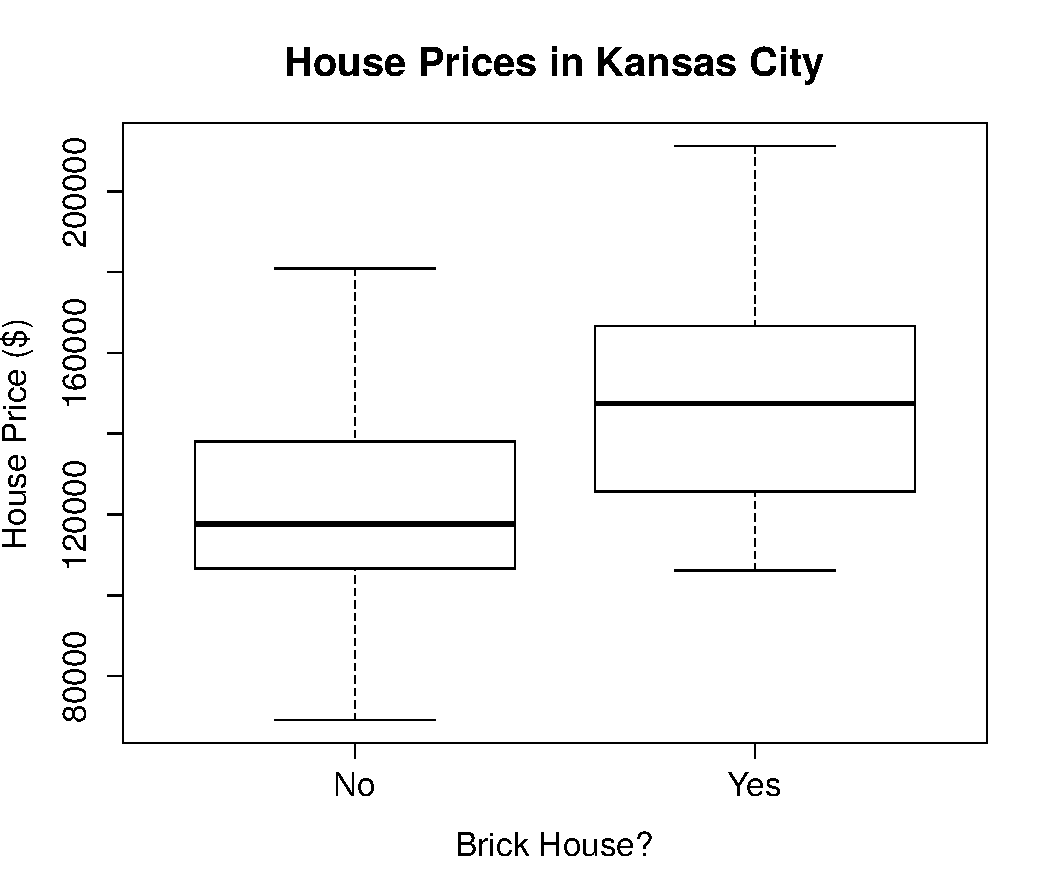
\includegraphics[scale=0.65]{finalDec2015_boxplot}\\
  \vspace{1em}
  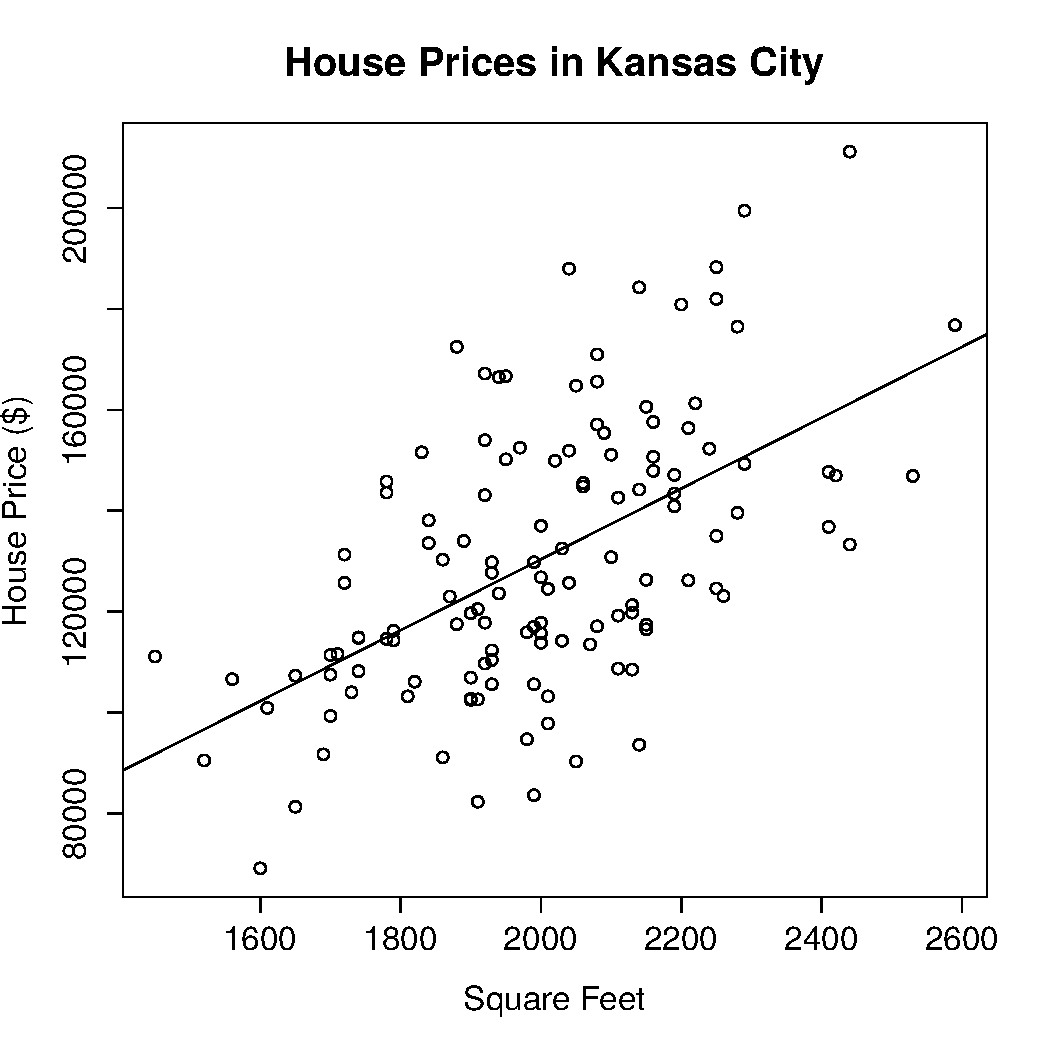
\includegraphics[scale=0.65]{finalDec2015_plot}
\end{figure}

\end{questions}


\end{document}
